\documentclass[tikz,border=15pt]{standalone}
\usepackage{amsmath,amssymb,bm}
\usepackage{tikz}
\usetikzlibrary{shapes.geometric, arrows.meta, positioning, calc, fit, backgrounds}

\begin{document}
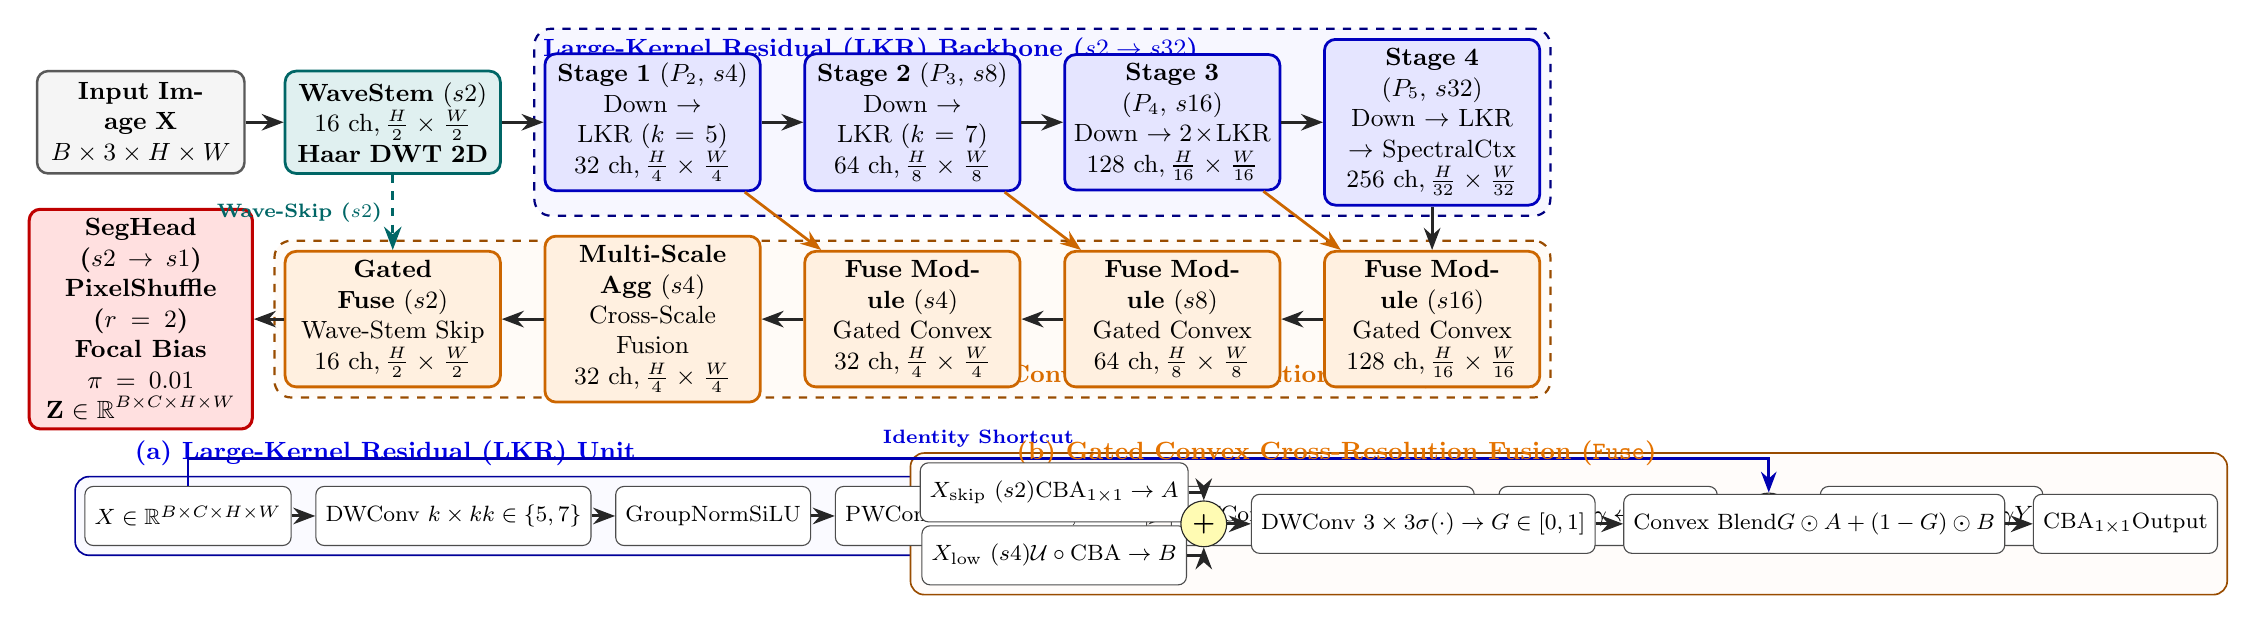
\begin{tikzpicture}[
    >=Stealth,
    font=\small,
    input_node/.style={rectangle, draw=gray!70!black, fill=gray!8, rounded corners=4pt, text width=2.4cm, text centered, minimum height=1.3cm, line width=0.9pt},
    stem_node/.style={rectangle, draw=teal!80!black, fill=teal!12, rounded corners=4pt, text width=2.5cm, text centered, minimum height=1.3cm, line width=1.0pt},
    bb_node/.style={rectangle, draw=blue!75!black, fill=blue!10, rounded corners=4pt, text width=2.5cm, text centered, minimum height=1.3cm, line width=1.0pt},
    neck_node/.style={rectangle, draw=orange!80!black, fill=orange!12, rounded corners=4pt, text width=2.5cm, text centered, minimum height=1.3cm, line width=1.0pt},
    head_node/.style={rectangle, draw=red!75!black, fill=red!12, rounded corners=4pt, text width=2.6cm, text centered, minimum height=1.3cm, line width=1.1pt, font=\small\bfseries},
    op_box/.style={rectangle, draw=black!70, fill=white, rounded corners=3pt, text centered, minimum height=0.75cm, inner sep=3.5pt, font=\footnotesize},
    circ_op/.style={circle, draw=black!85, fill=yellow!30, inner sep=2pt, font=\small\bfseries},
    fwd_arrow/.style={draw=black!85, -Stealth, line width=1.1pt},
    skip_arrow/.style={draw=teal!80!black, -Stealth, line width=1.2pt, dashed},
    lateral_arrow/.style={draw=orange!80!black, -Stealth, line width=1.0pt}
]
    % Top Row: Backbone Stages
    \node [input_node] (input) at (0, 0) {\textbf{Input Image} $\mathbf{X}$\\$B \times 3 \times H \times W$};
    \node [stem_node] (stem) at (3.2, 0) {\textbf{WaveStem} ($s2$)\\$16\text{ ch}, \frac{H}{2}\times\frac{W}{2}$\\\textbf{Haar DWT 2D}};
    \node [bb_node] (p2) at (6.5, 0) {\textbf{Stage 1} ($P_2$, $s4$)\\Down $\to$ LKR ($k=5$)\\$32\text{ ch}, \frac{H}{4}\times\frac{W}{4}$};
    \node [bb_node] (p3) at (9.8, 0) {\textbf{Stage 2} ($P_3$, $s8$)\\Down $\to$ LKR ($k=7$)\\$64\text{ ch}, \frac{H}{8}\times\frac{W}{8}$};
    \node [bb_node] (p4) at (13.1, 0) {\textbf{Stage 3} ($P_4$, $s16$)\\Down $\to 2\times\text{LKR}$\\$128\text{ ch}, \frac{H}{16}\times\frac{W}{16}$};
    \node [bb_node] (p5) at (16.4, 0) {\textbf{Stage 4} ($P_5$, $s32$)\\Down $\to$ LKR $\to$ SpectralCtx\\$256\text{ ch}, \frac{H}{32}\times\frac{W}{32}$};

    % Second Row: Gated Fusion Neck & Head
    \node [neck_node] (fuse16) at (16.4, -2.5) {\textbf{Fuse Module} ($s16$)\\Gated Convex\\$128\text{ ch}, \frac{H}{16}\times\frac{W}{16}$};
    \node [neck_node] (fuse8) at (13.1, -2.5) {\textbf{Fuse Module} ($s8$)\\Gated Convex\\$64\text{ ch}, \frac{H}{8}\times\frac{W}{8}$};
    \node [neck_node] (fuse4) at (9.8, -2.5) {\textbf{Fuse Module} ($s4$)\\Gated Convex\\$32\text{ ch}, \frac{H}{4}\times\frac{W}{4}$};
    \node [neck_node] (agg) at (6.5, -2.5) {\textbf{Multi-Scale Agg} ($s4$)\\Cross-Scale Fusion\\$32\text{ ch}, \frac{H}{4}\times\frac{W}{4}$};
    \node [neck_node] (fuse2) at (3.2, -2.5) {\textbf{Gated Fuse} ($s2$)\\Wave-Stem Skip\\$16\text{ ch}, \frac{H}{2}\times\frac{W}{2}$};
    \node [head_node] (head) at (0, -2.5) {\textbf{SegHead} ($s2 \to s1$)\\PixelShuffle ($r=2$)\\Focal Bias $\pi=0.01$\\$\mathbf{Z} \in \mathbb{R}^{B \times C \times H \times W}$};

    % Forward Backbone Connections
    \draw [fwd_arrow] (input) -- (stem);
    \draw [fwd_arrow] (stem) -- (p2);
    \draw [fwd_arrow] (p2) -- (p3);
    \draw [fwd_arrow] (p3) -- (p4);
    \draw [fwd_arrow] (p4) -- (p5);

    % Top-Down Neck Connections
    \draw [fwd_arrow] (p5) -- (fuse16);
    \draw [lateral_arrow] (p4) -- (fuse16);
    \draw [fwd_arrow] (fuse16) -- (fuse8);
    \draw [lateral_arrow] (p3) -- (fuse8);
    \draw [fwd_arrow] (fuse8) -- (fuse4);
    \draw [lateral_arrow] (p2) -- (fuse4);
    \draw [fwd_arrow] (fuse4) -- (agg);
    \draw [fwd_arrow] (agg) -- (fuse2);

    % High-Resolution Detail Skip from WaveStem to Stride s2 Fuse
    \draw [skip_arrow] (stem) -- (fuse2) node[midway, left, font=\scriptsize\bfseries, text=teal!80!black] {Wave-Skip ($s2$)};
    \draw [fwd_arrow] (fuse2) -- (head);

    % Background Scope Framing
    \begin{scope}[on background layer]
        \node [draw=blue!50!black, fill=blue!3, dashed, rounded corners=6pt, line width=0.8pt, fit=(p2) (p5), label={[font=\small\bfseries, text=blue!85!black, anchor=north west]north west:Large-Kernel Residual (LKR) Backbone ($s2 \to s32$)}] {};
        \node [draw=orange!60!black, fill=orange!3, dashed, rounded corners=6pt, line width=0.8pt, fit=(fuse16) (fuse2), label={[font=\small\bfseries, text=orange!85!black, anchor=south east]south east:Gated Convex Cross-Resolution Neck ($s32 \to s2$)}] {};
    \end{scope}

    % Micro Inset (a): Large-Kernel Residual (LKR) Block
    \node [anchor=west, font=\small\bfseries, text=blue!90!black] at (-0.2, -4.2) {(a) Large-Kernel Residual (LKR) Unit};
    \node [op_box] (lkr_in) at (0.6, -5.0) {$X \in \mathbb{R}^{B \times C \times H \times W}$};
    \node [op_box, right=0.3cm of lkr_in] (lkr_dw) {DWConv $k\times k$\\$k \in \{5, 7\}$};
    \node [op_box, right=0.3cm of lkr_dw] (lkr_gn1) {GroupNorm\\SiLU};
    \node [op_box, right=0.3cm of lkr_gn1] (lkr_pw1) {PWConv $1\times 1$\\$e=2.0$, SiLU};
    \node [op_box, right=0.3cm of lkr_pw1] (lkr_pw2) {PWConv $1\times 1$\\Project to $C$};
    \node [op_box, right=0.3cm of lkr_pw2] (lkr_scale) {GN $\times \gamma$\\($\gamma \leftarrow 0$ init)};
    \node [circ_op, right=0.35cm of lkr_scale] (lkr_add) {$\bm{+}$};
    \node [op_box, right=0.35cm of lkr_add] (lkr_out) {$\text{LKR}(X) = X + \gamma Y$};

    \draw [fwd_arrow] (lkr_in) -- (lkr_dw);
    \draw [fwd_arrow] (lkr_dw) -- (lkr_gn1);
    \draw [fwd_arrow] (lkr_gn1) -- (lkr_pw1);
    \draw [fwd_arrow] (lkr_pw1) -- (lkr_pw2);
    \draw [fwd_arrow] (lkr_pw2) -- (lkr_scale);
    \draw [fwd_arrow] (lkr_scale) -- (lkr_add);
    \draw [fwd_arrow] (lkr_add) -- (lkr_out);
    \draw [draw=blue!70!black, -Stealth, line width=1.0pt] (lkr_in.north) -- ++(0, 0.35) -| (lkr_add.north) node[pos=0.25, above, font=\scriptsize\bfseries, text=blue!85!black] {Identity Shortcut};

    % Micro Inset (b): Gated Convex Cross-Resolution Fusion
    \node [anchor=west, font=\small\bfseries, text=orange!90!black] at (11.0, -4.2) {(b) Gated Convex Cross-Resolution Fusion (\texttt{Fuse})};
    \node [op_box] (fuse_skip) at (11.6, -4.7) {$X_{\text{skip}}$ ($s2$)\\$\text{CBA}_{1\times 1} \to A$};
    \node [op_box] (fuse_low) at (11.6, -5.5) {$X_{\text{low}}$ ($s4$)\\$\mathcal{U} \circ \text{CBA} \to B$};
    
    \node [circ_op] (fuse_sum) at (13.5, -5.1) {$\bm{+}$};
    \node [op_box, right=0.3cm of fuse_sum] (fuse_gate) {DWConv $3\times 3$\\$\sigma(\cdot) \to G \in [0, 1]$};
    \node [op_box, right=0.35cm of fuse_gate] (fuse_blend) {Convex Blend\\$G \odot A + (1 - G) \odot B$};
    \node [op_box, right=0.35cm of fuse_blend] (fuse_out) {$\text{CBA}_{1\times 1}$\\Output};

    \draw [fwd_arrow] (fuse_skip.east) -| (fuse_sum.north);
    \draw [fwd_arrow] (fuse_low.east) -| (fuse_sum.south);
    \draw [fwd_arrow] (fuse_sum) -- (fuse_gate);
    \draw [fwd_arrow] (fuse_gate) -- (fuse_blend);
    \draw [fwd_arrow] (fuse_blend) -- (fuse_out);

    \begin{scope}[on background layer]
        \node [draw=blue!60!black, fill=blue!2, rounded corners=5pt, line width=0.6pt, fit=(lkr_in) (lkr_out) (lkr_dw) (lkr_scale)] {};
        \node [draw=orange!60!black, fill=orange!2, rounded corners=5pt, line width=0.6pt, fit=(fuse_skip) (fuse_low) (fuse_out) (fuse_gate)] {};
    \end{scope}
\end{tikzpicture}
\end{document}
